This is a 1-D problem that consists of a domain with 3 regions of differing
saturation values $q/\sigma$. An incident angular flux $u_{inc}$ enters the left
boundary. The first region has equal sink/source rates: $\sigma=q=u_{inc}=1$,
the second has a large cross section relative to the source: $\sigma=40,q=5$,
and the final region has equal sink/source rates again, but with different
values than the first region: $\sigma=q=20$.
This problem demonstrates the addition
of the reaction terms and source terms in the FCT methodology.

Figure \ref{fig:three_region} compares the solutions computed
for each scheme, using the 3-stage, 3rd-order SSPRK method.
Firstly one can see that the Galerkin solution is highly oscillatory. The
low-order solution is monotone and non-negative but very diffusive. The entropy
viscosity (EV) solution is much less oscillatory than the Galerkin solution,
but one can see there are still oscillations and negativities in the first
and second regions. Both the Galerkin FCT and the entropy-based FCT schemes
remedy these under/overshoots and negativities.

%-------------------------------------------------------------------------------
\begin{figure}[ht]
   \centering
   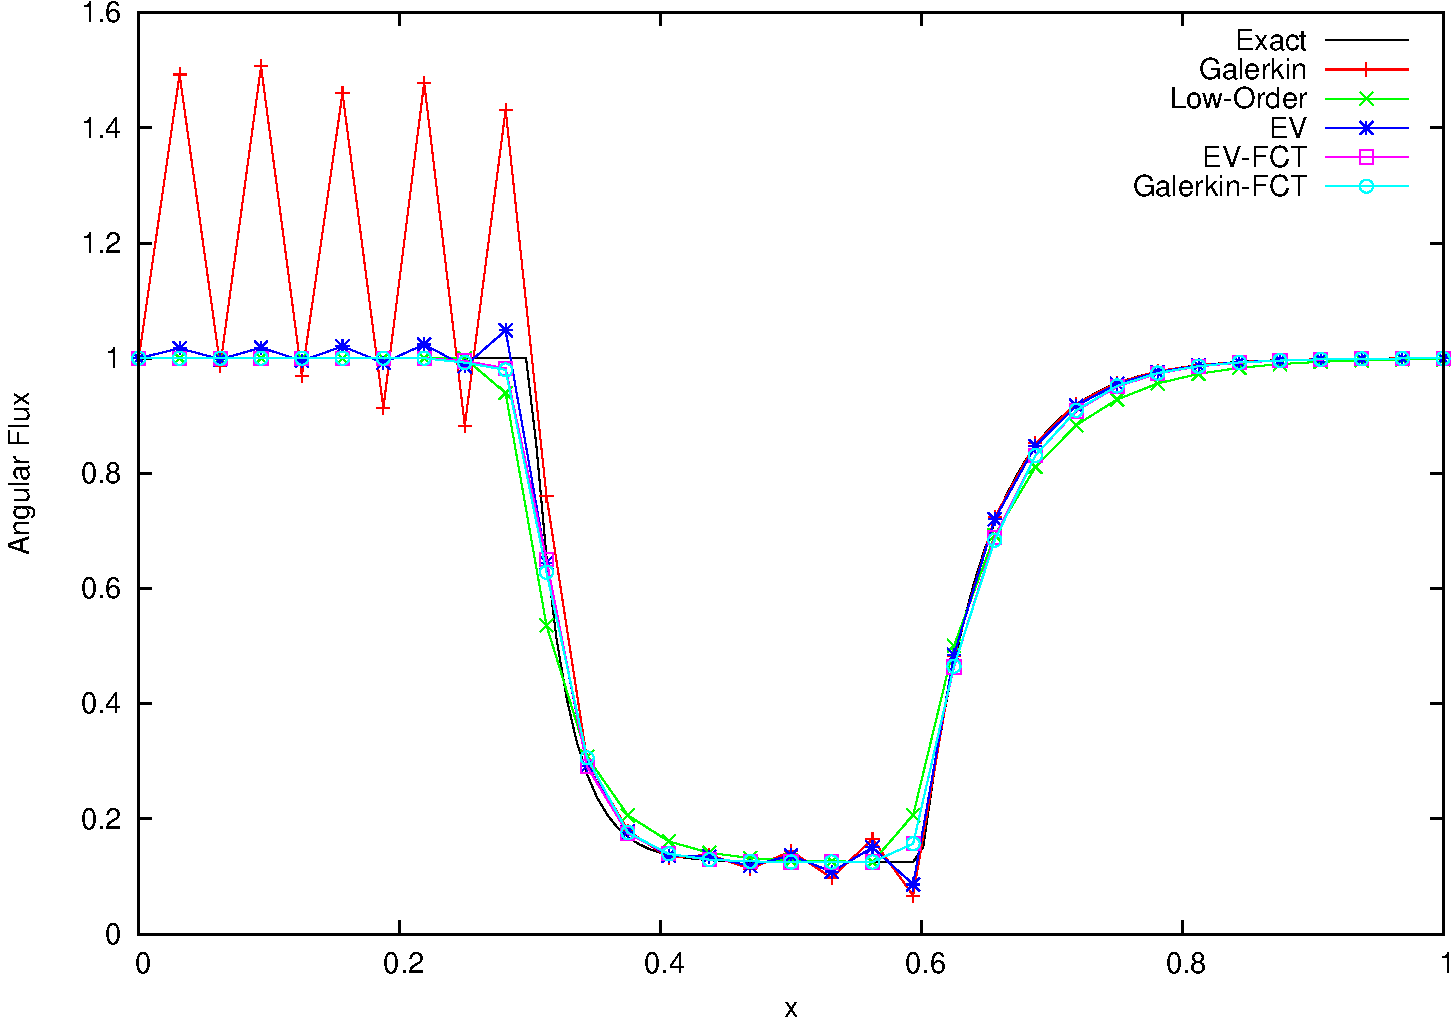
\includegraphics[width=0.9\textwidth]
     {\contentdir/results/transport/three_region/three_region.pdf}
   \caption{Comparison of Solutions for the 3-Region Test Problem}
   \label{fig:three_region}
\end{figure}
%-------------------------------------------------------------------------------
